\chapter{Privacy \& Security}
\label{ch:security}

There are several things you could and should pay attention to when you start your crypto-journey. An initial useful selection is provided in this chapter. Please feel free to check out all of our suggestions but don't forget that there are other alternatives out there that might be better for you, for whatever reason. Because of this, we've decided to keep it general and provide a link, a short description plus an example where possible.

\begin{quotation}

      \textit{\say{Holding and managing your own wealth comes with great responsibility. You - and you alone - are responsible for your own investments as there is no bank or other intermediary or third party involved in handling and safeguarding your assets.}}
      \begin{flushright}
        \small{--- \textbf{cryptomanuals.com}}
      \end{flushright}
    
\end{quotation}


\section{Threat modeling}
Threat modeling might sound a bit extreme, but it can be quite beneficial as it provides you with the opportunity to step back, assess the situation objectively and decide on your next steps in terms of protecting yourself. 

It involves several elements where you identify your online activities and the risks that might accompany those activities. Who might be interested in what you do online? What can you do to minimize that risk? It comes down to you creating a small risk matrix where you outline the potential dangers that might arise from your activities as an investor or a trader (or something else like your activities involving your job or hobbies for that matter). Most people don't stop and think about such things, and they go with the flow - thinking they'll be OK. What if you're not? Put in some effort to reduce or eliminate your risks by performing a brief analysis, based on your situation\footnote{AccessNow (13-06-2019); \href{https://www.accessnow.org/cms/assets/uploads/2019/08/Digital-Security-Start-Booklet-digital-Aug2019.pdf}{Digital Security}.}.

\section{Securely setting up mobile devices}
When you have installed wallet software on your phone and are carrying around a sum of cryptocurrencies, make sure your mobile phone is encrypted, is always locked and both your mobile and the specific software applications that you use to access your funds are secured with an active PIN. Biometrics such as fingerprint and face scanning is advised against as people with bad intentions can coerce you into unlocking your phone or wallet.

\section{Password managers}
It is highly advised to use a password manager extension (on both desktop and mobile) which generates ultra-safe passwords (up to 100 characters!) for you to use on both your crypto-related (exchange) accounts and personal accounts. LastPass provides local-only encryption of your password related data stored in your \say{vault} (extension to your browser). Your data is encrypted and decrypted at the device level. Data stored in your vault is kept a secret, even from LastPass. Your master password and the keys used to encrypt and decrypt data are never sent to their servers and are never accessible by LastPass. A password manager eliminates the reuse of old passwords and makes sure that you use unique and robust passwords.

    \bigskip
    \begin{tipbox}{\textbf{TIP}}
        Use Bitwarden, a free and open-source password manager which is very easy to oprate. Bitwarden generates strong passwords that are all encrypted. Weak passwords never need to be (re)used because only the end-user has access to this protected environment.
        \tcblower
        Go to \href{https://bitwarden.com/}{Bitwarden}.
    \end{tipbox}

\section{Two-Factor Authentication (2FA)}
\label{sec:2FA}

Two-factor authentication is a security mechanism that requires two types of credentials for authentication and is designed to provide an additional layer of validation, minimizing security breaches. Two-Factor authentication is also known as strong authentication. Two-Factor authentication works with two separate security or validation mechanisms. Typically, one is a physical validation token, and one is a valid code or password. Both must be validated before accessing a secured service or product. Generally, an authenticating procedure requires a physical token or identity validation, followed by a logical password or personal identification number (PIN). The security procedure for an ATM is a typical example of Two-Factor authentication, which requires that a user possesses a valid ATM card and PIN. The need for second layer security is undeniable and should be a part of everyone's login process to protect against phishing attacks, fraud, identity, and monetary theft.
\medskip

    \begin{tipbox}{\textbf{TIP}}
        In our case, you will most likely use your phone to download an application such as Google Authenticator (mobile device only) or Authy (mobile and desktop app). In this case, we recommend Authy since it offers a way to back up your codes on multiple devices in case you lose access to one of them (mobile, desktop or tablet). 
        \tcblower
        Go to \href{https://authy.com/}{Authy}.
    \end{tipbox}

\section{Virtual Private Networks (VPN)}
A Virtual Private Network (VPN) extends a private network across a public network and enables users to send and receive data across shared or public networks as if their computing devices were directly connected to the private network. Applications running across a VPN may, therefore, benefit from the functionality, security, and management of the private network. VPNs cannot make online connections completely anonymous, but they can usually increase privacy and security. To prevent disclosure of private information, VPNs typically allow only authenticated remote access using tunneling protocols and encryption techniques.

    \bigskip
    \begin{tipbox}{\textbf{TIP}}
        ProtonVPN offers excellent free and paid solutions, which come in tandem with their encrypted email services provided by ProtonMail. \tcblower
        Go to \href{https://protonmail.com/}{Protonmail}.
    \end{tipbox}

\section{Encrypted email services}
\href{https://protonmail.com/}{ProtonMail} offers a very nice alternative email service, and safety and security are an inherent aspect of their platform. It is open-source, anonymous, comes with Swiss privacy, all emails are protected by end-to-end encryption, and it is straightforward to use and pleasant on the eyes. Use a safe and dedicated email address for all things related to crypto and preferably set it up with 2FA and or a PIN.

\section{Encrypted messaging}
\emph{End-to-end} encryption keeps online conversations and calls secure. Nobody can eavesdrop and read any of your messages. Privacy is not an optional mode - it's just the way these applications work. Every message, every call and every time.\medskip

    \begin{tipbox}{TIP}
            As an alternative to the traditional messaging service WhatsApp, we recommend Signal. Signal enables fully encrypted messages, and offers numerous additional options for enhanced user privacy.
        \tcblower
        Have a look at \href{https://signal.org/}{Signal}.
    \end{tipbox}\medskip

\begin{borderbox}
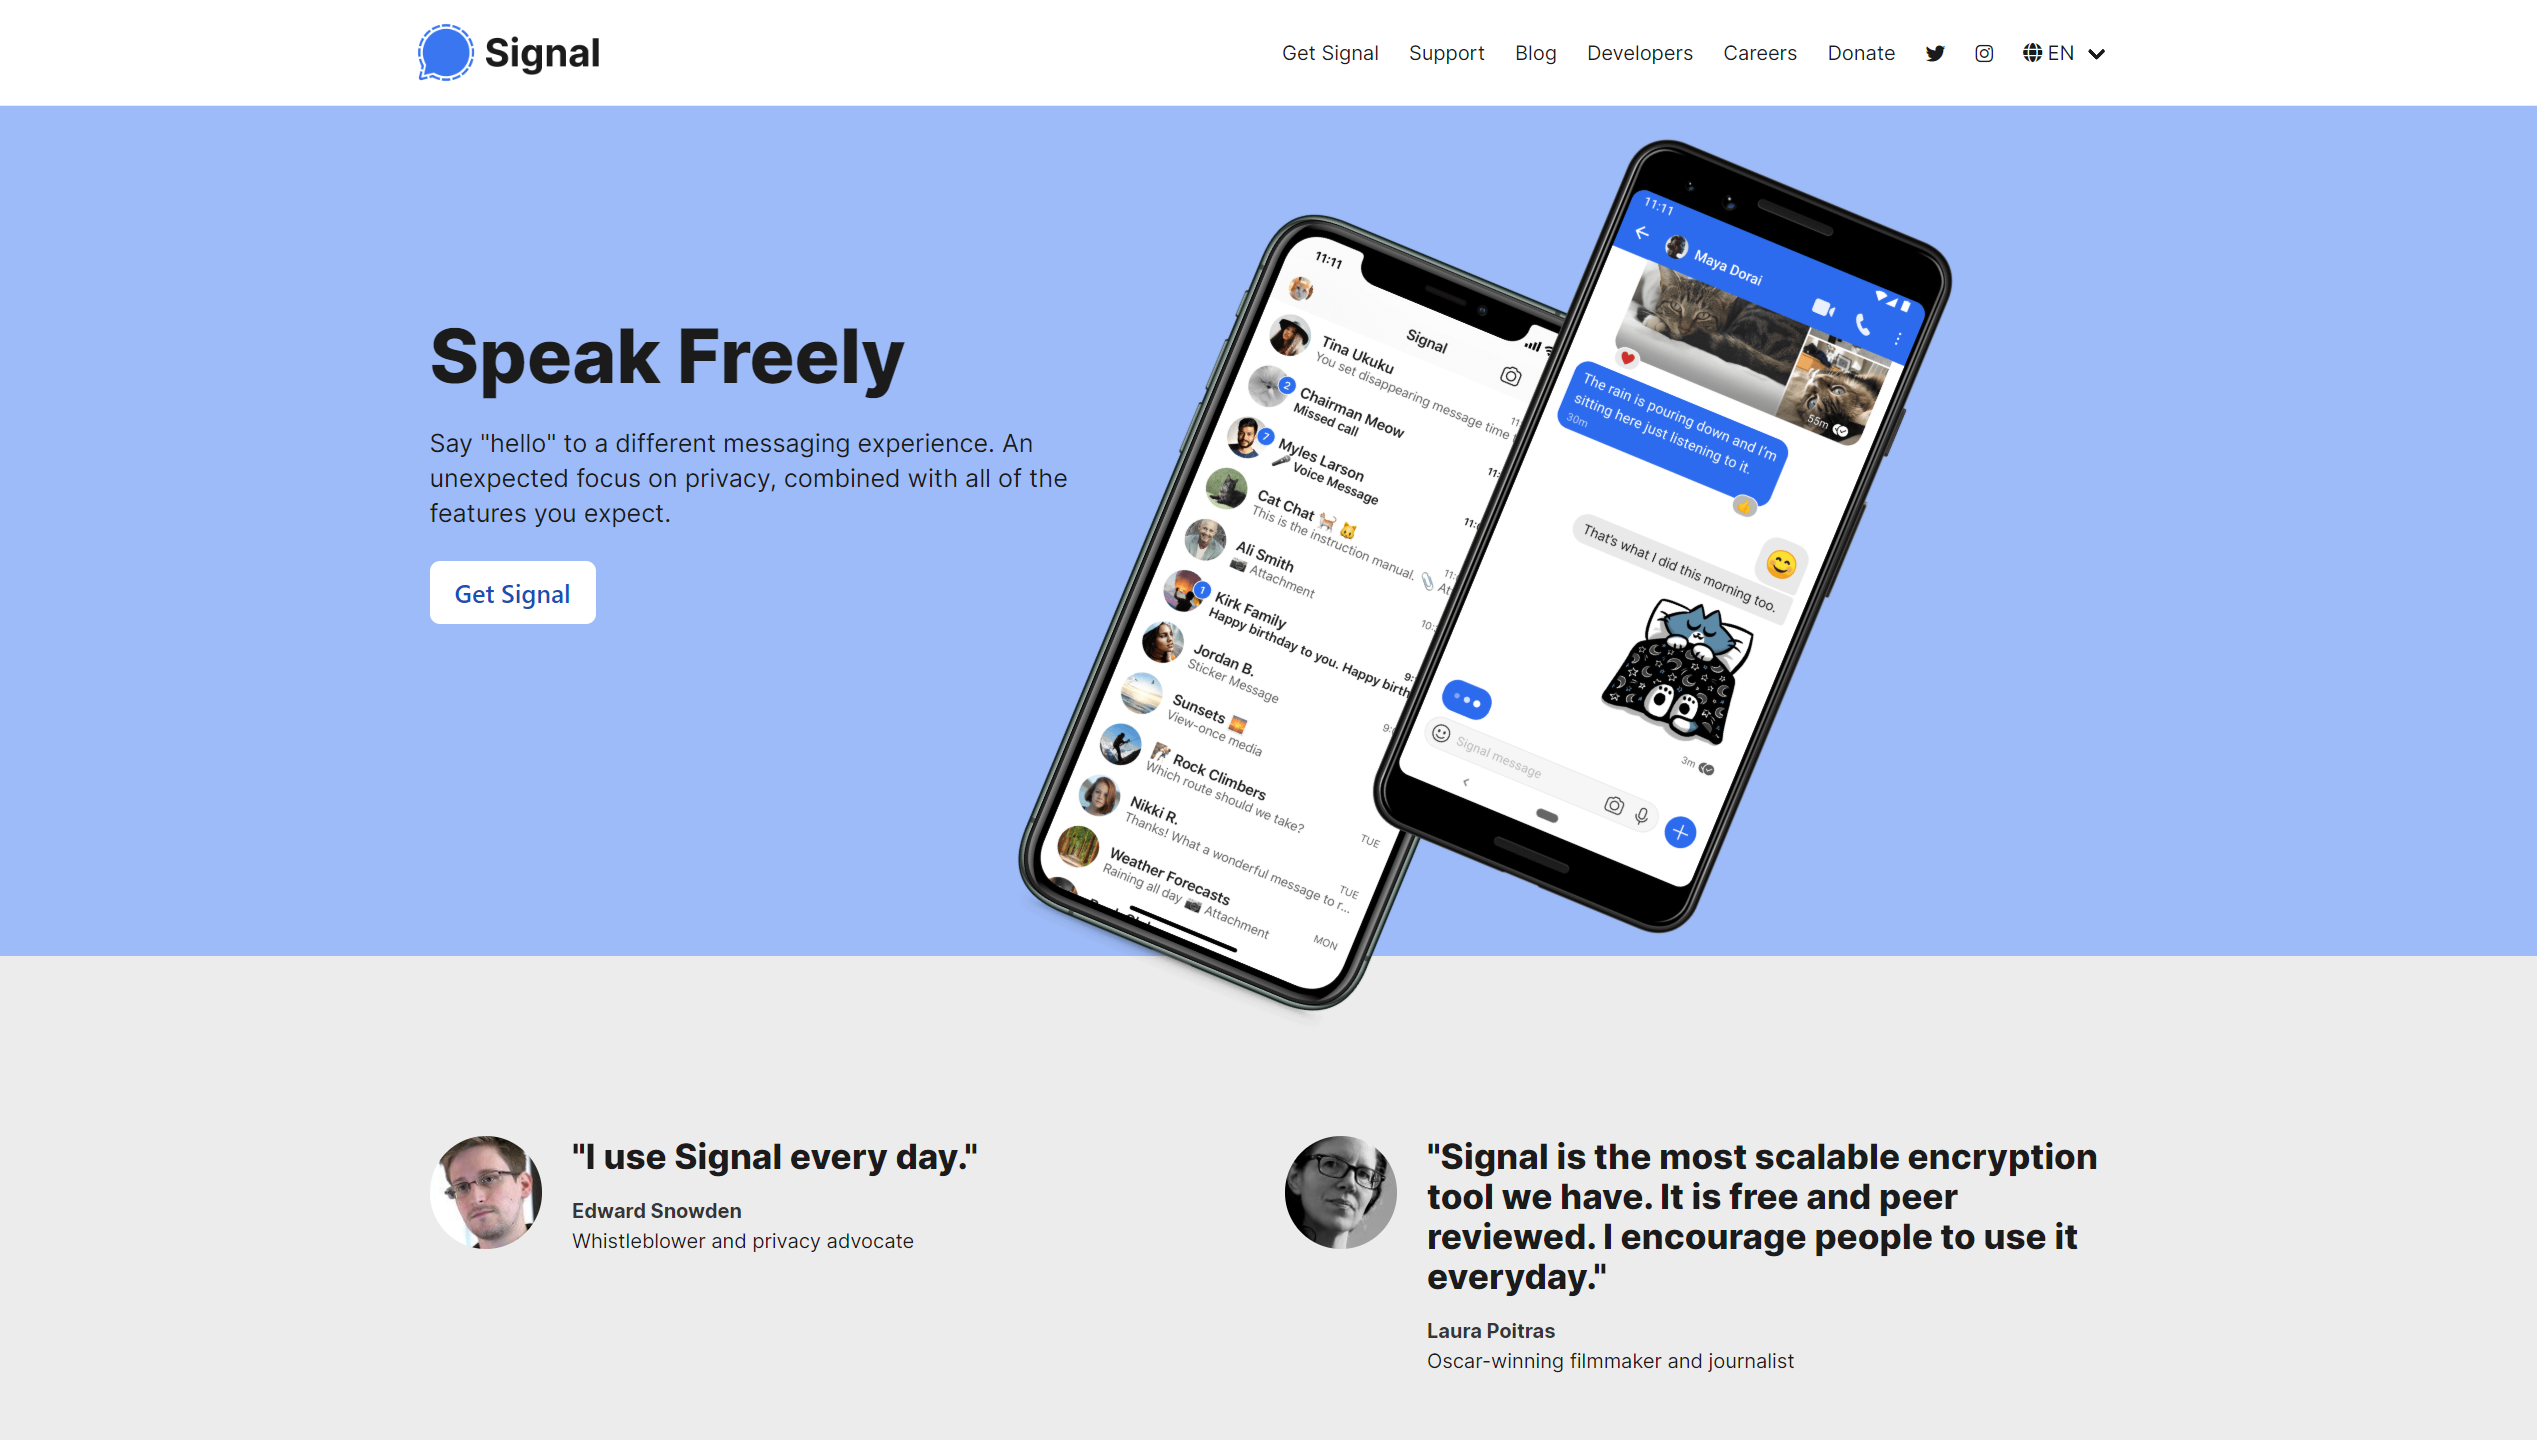
\includegraphics[width=\textwidth]{img/ch-privacy/signal.png}
\end{borderbox}


\section{Alternate internet browsers}
\href{https://brave.com/urm569}{Brave} offers you a completely new browsing experience, which does not track you online. Your browsing habits cannot be used to create an online shadow version of you, which is used to target ads against you. Your browsing experience will not only be faster and more secure but also private. Brave loads major news sites two to eight times faster than the leading browsers on mobile devices and two times faster on desktops. Brave automatically blocks all ads and trackers, which drastically improves loading speeds and increases the browsing experience. Brave also supports a blockchain-based token called the Basic Attention Token (BAT) which allows the user to tip their favorite content creators. Being much more than a browser, Brave is a new way of thinking about how the web works, enabling micro-transactions and one step closer toward a new internet of value. Brave is open source, and built by a team of privacy focused, performance oriented pioneers of the web, founded by the inventor of JavaScript and co-founder of Mozilla.

\begin{quotation}
       \textit{\say{If you are not paying for your product, you very well might \emph{\textbf{be}} the product.}}
\end{quotation}

    \begin{tipbox}{\textbf{TIP}}
        Brave uses the cryptocurrency BAT (Basic Attention Token) which allows users to tip their favorite websites and content creators. You can also earn crypto while browsing and using the internet. 
        \tcblower
        Learn more? Go to \href{https://brave.com/urm569}{Brave}.
    \end{tipbox}

\section{Private search engines}
DuckDuckGo is a search engine extension application, which is already implemented in the Brave browser but also usable in Chrome. DuckDuckGo doesn't collect or share any of your personal information and doesn't store your search history. Therefore, they have nothing to sell to advertisers that track you across the internet. Whereas other search engines can also track you in private browsing mode, DuckDuckGo never tracks users.

    \bigskip
    \begin{tipbox}{\textbf{TIP}}
        DuckDuckGo is a search engine extension and application (built-in Brave). It does not collect or share personal information and does not store your search history. As a result, it has no data to sell to advertisers who are tracking you over the Internet. While other search engines can still track you in private browsing mode, DuckDuckGo \emph{never} tracks users.
        \tcblower
        Checkout \href{https://duckduckgo.com/}{DuckDuckGo}.
    \end{tipbox}
    \bigskip

\section{Software updates}
Software updates include but are not limited to wallet software. Also think about anti-virus software, spyware, and malware software, windows updates, mobile wallet applications, etc. Exchanges provide you with a wallet that you have no direct control over (no access to private keys) and you don't need to update these. Keep your PC or mobile up to date on security packages and external (wallet or exchange) software offered by the official developers on your mobile device or your desktop.

\section{Backup sensitive data}
Even if you have a password manager, it is always recommended to have at least one copy (or printout) of your passwords, private keys, passwords, PINs or seed phrases in a safe location. If for any reason you lose access to your mobile, or your desktop computer breaks down, you can access your funds from another device and restore your respective wallets with your backup. Ultimately, the best method of storing your sensitive login information is by thinking of as many bad scenarios as you can think of and plan accordingly, creating redundancy. For instance, it is completely ill-advised storing your data on a note-taking app, computer, cloud storage, Google Drive, or Dropbox due to the risk of your computer or the centralized firm that keeps your data being hacked and your seed stolen. Even something written on a piece of paper might be lost due to one of the following; the ink might fade, the house might burn down, burglars might steal your files or deposit box, friends or family might (accidentally) take it, and the list goes on and on. Think about these implications.\medskip

The gravity of this must not go unnoticed as many people fall victim to security breaches every week for many reasons. They could have had their cryptocurrencies on an exchange wallet, which got hacked. They could have forgotten to set up 2FA. They could have used weak passwords, they could have accidentally used a phishing website which stole their login details, and the list goes on. 

\section{Data phishing}
Finally, you can throw as much software at your threats as you want, but privacy and security are still contingent on human error. If you get hacked, all the encryption in the world won't protect you. The origin of a hack can often be traced back to an individual clicking on a malicious link or unknowingly downloading malware from an email - such attacks are called phishing. There are plenty of prime examples of phishing attacks out there, and we advise you to browse your spam folder if you're unsure what phishing might look like as you will find plenty examples in your inbox.\medskip

    \begin{tipbox}{\textbf{TIP}}
        If a proposition sounds too good to be true? Be careful, as this is true for 99\% of all cases! Be extra cautious when you are asked to click on some unknown link or log into an account in order to claim free crypto or a reward of any kind. Remember the points identified below.
        \tcblower
        Learn more at \href{https://www.securitymetrics.com/blog/7-ways-recognize-phishing-email}{Securitymetrics}.
    \end{tipbox}
    \bigskip

Legit online activities will \emph{\textbf{always}}:

\begin{enumerate}[label=(\alph*)]
  \setlength\itemsep{0em}
    \item ... call customers by their name.
    \item ... use their own, company-related domain names.
    \item ... use correct language and grammar.
\end{enumerate}

Legit online activities will \emph{\textbf{never}}:

\begin{enumerate}[label=(\alph*)]
  \setlength\itemsep{0em}
    \item ... request sensitive information via e-mail.
    \item ... give away vast amounts of free crypto on social media or other platforms.
    \item ... try to persuade people to click on buttons and links to get important information.
    \item ... send unsolicited attachments.
\end{enumerate}

The information in this e-manual is intended to help you enter the market with the required basic knowledge and tools to keep it as safe as you possibly can. Don't be irresponsible, take the topic of online safety seriously, even beyond the cryptocurrency space.If you act carelessly in terms of security, you expose yourself to unnecessary risks and increase the chances of your funds being compromised.

\begin{quotation}

      \textit{\say{As you are your own bank(er), you - and you alone - are responsible for your investments.}}
        \begin{flushright}
        \small{--- \textbf{cryptomanuals}}
      \end{flushright}
\end{quotation}
    
\medskip
